\section{Verification}
\label{section: Chapter3/verification}

%%%%%%%%%%%%%%%%%%%%%%%%%%%%%%%%%%%%%%%%%%%%%%%%%%%%%%%%%%%%%%%%%%%%%%%%%%%%%%%%%%%%%%%%%%%
%%%%%%%%%%%%%%%%%%%%%%%%%%%%%%%%%%%%%%%%%%%%%%%%%%%%%%%%%%%%%%%%%%%%%%%%%%%%%%%%%%%%%%%%%%%
%%%%%%%%%%%%%%%%%%%%%%%%%%%%%%%%%%%%%%%%%%%%%%%%%%%%%%%%%%%%%%%%%%%%%%%%%%%%%%%%%%%%%%%%%%%
%%%%%%%%%%%%%%%%%%%%%%%%%%%%%%%%%%%%%%%%%%%%%%%%%%%%%%%%%%%%%%%%%%%%%%%%%%%%%%%%%%%%%%%%%%%
%%%%%%%%%%%%%%%%%%%%%%%%%%%%%%%%%%%%%%%%%%%%%%%%%%%%%%%%%%%%%%%%%%%%%%%%%%%%%%%%%%%%%%%%%%%
%%%%%%%%%%%%%%%%%%%%%%%%%%%%%%%%%%%%%%%%%%%%%%%%%%%%%%%%%%%%%%%%%%%%%%%%%%%%%%%%%%%%%%%%%%%
%%%%%%%%%%%%%%%%%%%%%%%%%%%%%%%%%%%%%%%%%%%%%%%%%%%%%%%%%%%%%%%%%%%%%%%%%%%%%%%%%%%%%%%%%%%
%%%%%%%%%%%%%%%%%%%%%%%%%%%%%%%%%%%%%%%%%%%%%%%%%%%%%%%%%%%%%%%%%%%%%%%%%%%%%%%%%%%%%%%%%%%
%%%%%%%%%%%%%%%%%%%%%%%%%%%%%%%%%%%%%%%%%%%%%%%%%%%%%%%%%%%%%%%%%%%%%%%%%%%%%%%%%%%%%%%%%%%
%%%%%%%%%%%%%%%%%%%%%%%%%%%%%%%%%%%%%%%%%%%%%%%%%%%%%%%%%%%%%%%%%%%%%%%%%%%%%%%%%%%%%%%%%%%
\subsection{Uniaxial traction of a bar}
\label{section: Chapter3/verification/bar}

We first verify the uniaxial response of the quasi-brittle fracture model with a pressurized crack. Consider a bar of length $2L = \SI{400}{\milli\meter}$ and width $2W = \SI{2}{\milli\meter}$ that is subject to uniaxial tension. Plane strain conditions are assumed to hold. A similar example without crack pressurization can be found in \cite{JYWu2017}. Boundary conditions are shown in \Cref{fig:bar}. Both ends of the bar are subject to monotonically increasing horizontal displacements. Only a quarter of the domain is simulated utilizing the two symmetry conditions. The domain is uniformly discretized using \texttt{QUAD4} elements, with 200 elements along the length and 1 element along the width.
The material and model parameters are Young's modulus $E = \SI{3e4}{\mega\pascal}$, Poisson's ratio $\nu = 0.2$, critical fracture strength $\psi_c = \SI{1.5e-4}{\milli\joule\per\cubic\milli\meter}$, fracture toughness $\Gc = \SI{0.12}{\milli\joule\per\square\milli\meter}$, and the characteristic length $l_\text{ch} = \dfrac{\Gc}{2\psi_c} = \SI{400}{\milli\meter}$.

\begin{figure}[!ht]
  \centering
  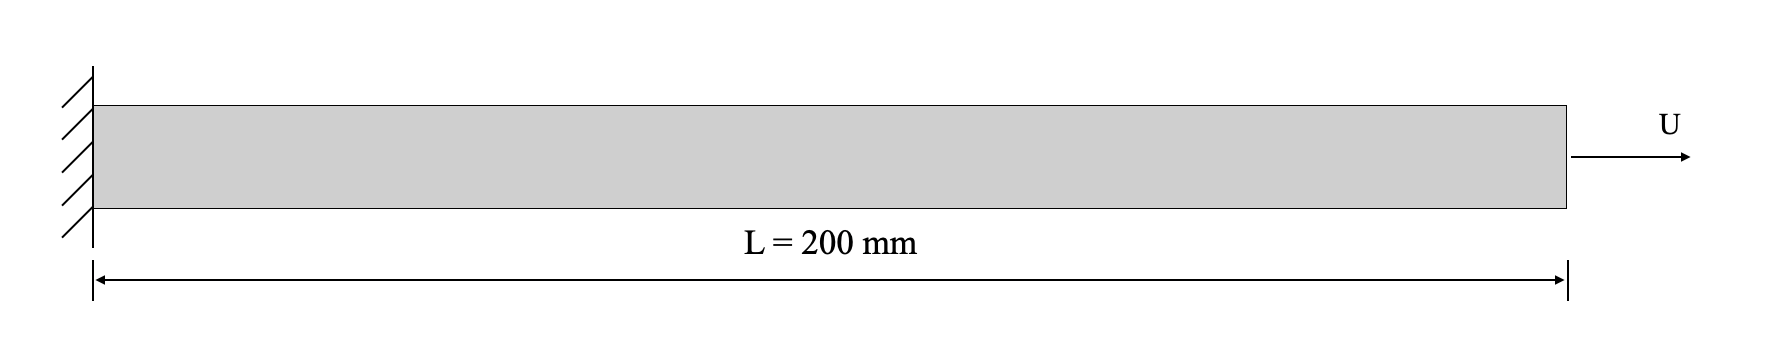
\includegraphics[width=0.9\textwidth,trim={0 8cm 0 8cm},clip]{Chapter3/figures/bar}
  \caption{A bar under uniaxial tension.}
  \label{fig:bar}
\end{figure}

An arbitrarily small imperfection, $d_0 = \mathcal{O}(\epsilon)$, is introduced on the left side of the computational domain to induce localization.
To study the effect of the pressure, different pressure values
\begin{align*}
  \bar{p} \in \left\{ \SI{0}{\mega\pascal}, \SI{0.25}{\mega\pascal}, \SI{0.5}{\mega\pascal}, \SI{0.75}{\mega\pascal}, \SI{1}{\mega\pascal} \right\}
\end{align*}
are considered. In the context of fuel fracture, the pressure on the crack surfaces can result from a pressurized gas environment.

\begin{figure}[htbp!]
  \centering
  \begin{subfigure}[b]{0.95\textwidth}
    \centering
    \tikzsetnextfilenamesafe{Chapter3/verification/compare_ts/p}
    \begin{tikzpicture}[spy using outlines={rectangle, magnification=3, width=10cm, height=2cm, connect spies}]
      \begin{axis}[
          colormap/jet,
          cycle list={[of colormap,samples of colormap=5]},
          width=\textwidth,
          height=0.6\textwidth,
          xmin=0,
          xmax=0.1,
          ymin=0,
          xlabel=$w$ (\SI{}{\milli\meter}),
          ylabel=$t$ (\SI{}{\newton}),
          scaled x ticks=false,
          yticklabel style={
              /pgf/number format/fixed,
              /pgf/number format/precision=2
            },
          xticklabel style={
              /pgf/number format/fixed,
              /pgf/number format/precision=2
            },
          legend style={
              at={(0.97,0.97)},
              anchor=north east,
              nodes={scale=1, transform shape},
              fill=none,
              draw=none,
              text opacity=1,
              cells={align=left}
            },
          legend cell align={left},
          every axis plot/.append style={no marks}
        ]
        \addplot table[x=separation,y expr=-\thisrowno{1},col sep=comma]{Chapter3/data/force_disp_p_0_r_5.csv};
        \addplot table[x=separation,y expr=-\thisrowno{1},col sep=comma]{Chapter3/data/force_disp_p_0.25_r_5.csv};
        \addplot table[x=separation,y expr=-\thisrowno{1},col sep=comma]{Chapter3/data/force_disp_p_0.5_r_5.csv};
        \addplot table[x=separation,y expr=-\thisrowno{1},col sep=comma]{Chapter3/data/force_disp_p_0.75_r_5.csv};
        \addplot table[x=separation,y expr=-\thisrowno{1},col sep=comma]{Chapter3/data/force_disp_p_1_r_5.csv};
        \coordinate (spypoint) at (axis cs:0.05,0.175);
        \coordinate (magnifyglass) at (axis cs:0.06,1.5);
        \legend{$p=\SI{0}{\mega\pascal}$,$p=\SI{0.25}{\mega\pascal}$,$p=\SI{0.5}{\mega\pascal}$,$p=\SI{0.75}{\mega\pascal}$,$p=\SI{1}{\mega\pascal}$}
      \end{axis}
      \spy [black] on (spypoint) in node[fill=white] at (magnifyglass);
    \end{tikzpicture}
    \caption{}
    \label{fig: Chapter3/verification/compare_ts/p}
  \end{subfigure}
  
  \begin{subfigure}[b]{0.95\textwidth}
    \centering
    \tikzsetnextfilenamesafe{Chapter3/verification/compare_ts/l}
    \begin{tikzpicture}[spy using outlines={rectangle, magnification=3, width=2cm, height=5cm, connect spies}]
      \begin{axis}[
          colormap/jet,
          cycle list={[of colormap,samples of colormap=5]},
          width=\textwidth,
          height=0.6\textwidth,
          xmin=0,
          xmax=0.1,
          ymin=0,
          xlabel=$w$ (\SI{}{\milli\meter}),
          ylabel=$t$ (\SI{}{\newton}),
          scaled x ticks=false,
          yticklabel style={
              /pgf/number format/fixed,
              /pgf/number format/precision=2
            },
          xticklabel style={
              /pgf/number format/fixed,
              /pgf/number format/precision=2
            },
          legend style={
              at={(0.97,0.97)},
              anchor=north east,
              nodes={scale=1, transform shape},
              fill=none,
              draw=none,
              text opacity=1,
              cells={align=left}
            },
          legend cell align={left},
          every axis plot/.append style={no marks}
        ]
        \addplot table[x=separation,y expr=-\thisrowno{1},col sep=comma]{Chapter3/data/force_disp_p_0.25_r_5_l_2.csv};
        \addplot table[x=separation,y expr=-\thisrowno{1},col sep=comma]{Chapter3/data/force_disp_p_0.25_r_5_l_5.csv};
        \addplot table[x=separation,y expr=-\thisrowno{1},col sep=comma]{Chapter3/data/force_disp_p_0.25_r_5_l_10.csv};
        \addplot table[x=separation,y expr=-\thisrowno{1},col sep=comma]{Chapter3/data/force_disp_p_0.25_r_5_l_20.csv};
        \addplot table[x=separation,y expr=-\thisrowno{1},col sep=comma]{Chapter3/data/force_disp_p_0.25_r_5_l_50.csv};
        \coordinate (spypoint) at (axis cs:0.008,1.75);
        \coordinate (magnifyglass) at (axis cs:0.06,1.5);
        \legend{$l=\SI{2}{\milli\meter}$,$l=\SI{5}{\milli\meter}$,$l=\SI{10}{\milli\meter}$,$l=\SI{20}{\milli\meter}$,$l=\SI{50}{\milli\meter}$}
      \end{axis}
      \spy [black] on (spypoint) in node[fill=white] at (magnifyglass);
    \end{tikzpicture}
    \caption{}
    \label{fig: Chapter3/verification/compare_ts/l}
  \end{subfigure}
  \caption[The apparent traction-separation relations.]{The apparent traction-separation relations (a) for different values of pressure with a fixed regularization length $l = \SI{5}{\milli\meter}$ and (b) for different values of regularization length with a fixed pressure $p = \SI{0.25}{\mega\pascal}$. The level of mesh refinement is chosen to be $l / h^e = 5$. }
\end{figure}


\Cref{fig: Chapter3/verification/compare_ts/p} plots the apparent traction-separation law. The traction $t$ and the separation $w$ are approximated as $t = -R_x^\text{left}$ and $w = - \int\limits_{\body_0} \btu \cdot \grad I \diff{V}$, respectively. The apparent traction separation relations for different values of pressure are virtually indistinguishable.
\begin{remark}
  In similar formulations of pressurized crack using phase-field (e.g. \cite{CHUKWUDOZIE2019957,Mikeli__2015,WILSON2016264}), the fact that the pressure work (or the pressure power in the current variational framework) is independent of the velocities of the phase-field, i.e. $\dot{d}, \grad \dot{d}$, is not respected. Leading to formulations of the following form:
  \begin{subequations}
    \begin{align}
      \divergence \stress - \bar{p} \grad d I_{,d} & = \bs{0}, \\
      \divergence \bs{\xi} - f                     & = 0,      
    \end{align}
  \end{subequations}
  where
  \begin{align}
    \bs{\xi} = \dfrac{2\Gc l}{c_0} \grad d, \quad f = g_{,d}\psi^e_\activepart - \bar{p}\divergence\btu + \dfrac{\Gc}{c_0l}\alpha_{,d}.
  \end{align}
  Note that an additional contribution from the pressure arises in $f$, which leads to pressure-dependent traction-separation relations and critical fracture strength.
\end{remark}
At a given load (prescribed displacement), with a larger pressure, the separation between the crack surfaces is larger, resulting in a smaller traction. \Cref{fig: Chapter3/verification/compare_ts/l} shows the convergence of the apparent traction-separation law as $l \to 0$.

\begin{figure}[htbp!]
  \captionsetup{font=footnotesize}
  \centering
  \begin{subfigure}[b]{0.31\textwidth}
    \caption*{$R_x^\text{left}$ (\SI{}{\newton})}
  \end{subfigure}
  \begin{subfigure}[b]{0.31\textwidth}
    \caption*{$R_x^\text{right}$ (\SI{}{\newton})}
  \end{subfigure}
  \begin{subfigure}[b]{0.31\textwidth}
    \caption*{$\widetilde{p}$ (\SI{}{\mega\pascal})}
  \end{subfigure}
  %%%%%%%%%%%%%%%%%%%%%%%%%%%%%%%%%%%%%%%%%%%%%%%%%%%%%%%%%%%%%%%%%%%%%%%%%%%%%%%%%%%%%%%%%%%
  %%%%%%%%%%%%%%%%%%%%%%%%%%%%%%%%%%%%%%%%%%%%%%%%%%%%%%%%%%%%%%%%%%%%%%%%%%%%%%%%%%%%%%%%%%%
  %%%%%%%%%%%%%%%%%%%%%%%%%%%%%%%%%%%%%%%%%%%%%%%%%%%%%%%%%%%%%%%%%%%%%%%%%%%%%%%%%%%%%%%%%%%
  %%%%%%%%%%%%%%%%%%%%%%%%%%%%%%%%%%%%%%%%%%%%%%%%%%%%%%%%%%%%%%%%%%%%%%%%%%%%%%%%%%%%%%%%%%%
  %%%%%%%%%%%%%%%%%%%%%%%%%%%%%%%%%%%%%%%%%%%%%%%%%%%%%%%%%%%%%%%%%%%%%%%%%%%%%%%%%%%%%%%%%%%
  %%%%%%%%%%%%%%%%%%%%%%%%%%%%%%%%%%%%%%%%%%%%%%%%%%%%%%%%%%%%%%%%%%%%%%%%%%%%%%%%%%%%%%%%%%%
  %%%%%%%%%%%%%%%%%%%%%%%%%%%%%%%%%%%%%%%%%%%%%%%%%%%%%%%%%%%%%%%%%%%%%%%%%%%%%%%%%%%%%%%%%%%
  %%%%%%%%%%%%%%%%%%%%%%%%%%%%%%%%%%%%%%%%%%%%%%%%%%%%%%%%%%%%%%%%%%%%%%%%%%%%%%%%%%%%%%%%%%%
  %%%%%%%%%%%%%%%%%%%%%%%%%%%%%%%%%%%%%%%%%%%%%%%%%%%%%%%%%%%%%%%%%%%%%%%%%%%%%%%%%%%%%%%%%%%
  %%%%%%%%%%%%%%%%%%%%%%%%%%%%%%%%%%%%%%%%%%%%%%%%%%%%%%%%%%%%%%%%%%%%%%%%%%%%%%%%%%%%%%%%%%%
  % r = 5
  
  \begin{subfigure}[b]{0.31\textwidth}
    \centering
    \tikzsetnextfilenamesafe{Chapter3/verification/compare_r/Rx_left_r_5}
    \begin{tikzpicture}
      \begin{axis}[
          colormap/jet,
          cycle list={[of colormap,samples of colormap=5]},
          width=\textwidth,
          height=0.75\textwidth,
          xmin=0,
          xmax=0.05,
          ymin=-3.2,
          ymax=0,
          scaled x ticks=false,
          yticklabel style={
              /pgf/number format/fixed,
              /pgf/number format/precision=2
            },
          xticklabel style={
              /pgf/number format/fixed,
              /pgf/number format/precision=2
            },
          legend style={
              at={(1,0)},
              anchor=south east,
              nodes={scale=0.4, transform shape},
              fill=none,
              draw=none,
              text opacity=1,
              cells={align=left}
            },
          legend cell align={left},
          every axis plot/.append style={thick,no marks}
        ]
        \addplot table[x=time,y=Rx_left,col sep=comma]{Chapter3/data/force_disp_p_0_r_5.csv};
        \addplot table[x=time,y=Rx_left,col sep=comma]{Chapter3/data/force_disp_p_0.25_r_5.csv};
        \addplot table[x=time,y=Rx_left,col sep=comma]{Chapter3/data/force_disp_p_0.5_r_5.csv};
        \addplot table[x=time,y=Rx_left,col sep=comma]{Chapter3/data/force_disp_p_0.75_r_5.csv};
        \addplot table[x=time,y=Rx_left,col sep=comma]{Chapter3/data/force_disp_p_1_r_5.csv};
        \legend{$p=\SI{0}{\mega\pascal}$,$p=\SI{0.25}{\mega\pascal}$,$p=\SI{0.5}{\mega\pascal}$,$p=\SI{0.75}{\mega\pascal}$,$p=\SI{1}{\mega\pascal}$}
      \end{axis}
    \end{tikzpicture}
    \caption{$l/h^e = 5$}
    \label{fig: Chapter3/verification/compare_r/Rx_left_r_5}
  \end{subfigure}
  \begin{subfigure}[b]{0.31\textwidth}
    \centering
    \tikzsetnextfilenamesafe{Chapter3/verification/compare_r/Rx_right_r_5}
    \begin{tikzpicture}
      \begin{axis}[
          colormap/jet,
          cycle list={[of colormap,samples of colormap=5]},
          width=\textwidth,
          height=0.75\textwidth,
          xmin=0,
          xmax=0.05,
          ymin=-1.2,
          ymax=3.2,
          scaled x ticks=false,
          yticklabel style={
              /pgf/number format/fixed,
              /pgf/number format/precision=2
            },
          xticklabel style={
              /pgf/number format/fixed,
              /pgf/number format/precision=2
            },
          every axis plot/.append style={thick,no marks}
        ]
        \addplot table[x=time,y=Rx_right,col sep=comma]{Chapter3/data/force_disp_p_0_r_5.csv};
        \addplot table[x=time,y=Rx_right,col sep=comma]{Chapter3/data/force_disp_p_0.25_r_5.csv};
        \addplot table[x=time,y=Rx_right,col sep=comma]{Chapter3/data/force_disp_p_0.5_r_5.csv};
        \addplot table[x=time,y=Rx_right,col sep=comma]{Chapter3/data/force_disp_p_0.75_r_5.csv};
        \addplot table[x=time,y=Rx_right,col sep=comma]{Chapter3/data/force_disp_p_1_r_5.csv};
      \end{axis}
    \end{tikzpicture}
    \caption{$l/h^e = 5$}
    \label{fig: Chapter3/verification/compare_r/Rx_right_r_5}
  \end{subfigure}
  \begin{subfigure}[b]{0.31\textwidth}
    \centering
    \tikzsetnextfilenamesafe{Chapter3/verification/compare_r/p_r_5}
    \begin{tikzpicture}
      \begin{axis}[
          colormap/jet,
          cycle list={[of colormap,samples of colormap=5]},
          width=\textwidth,
          height=0.75\textwidth,
          xmin=0,
          xmax=0.05,
          ymin=-0.2,
          ymax=1.2,
          scaled x ticks=false,
          yticklabel style={
              /pgf/number format/fixed,
              /pgf/number format/precision=2
            },
          xticklabel style={
              /pgf/number format/fixed,
              /pgf/number format/precision=2
            },
          every axis plot/.append style={thick,no marks}
        ]
        \addplot table[x=time,y=p,col sep=comma]{Chapter3/data/force_disp_p_0_r_5.csv};
        \addplot table[x=time,y=p,col sep=comma]{Chapter3/data/force_disp_p_0.25_r_5.csv};
        \addplot table[x=time,y=p,col sep=comma]{Chapter3/data/force_disp_p_0.5_r_5.csv};
        \addplot table[x=time,y=p,col sep=comma]{Chapter3/data/force_disp_p_0.75_r_5.csv};
        \addplot table[x=time,y=p,col sep=comma]{Chapter3/data/force_disp_p_1_r_5.csv};
      \end{axis}
    \end{tikzpicture}
    \caption{$l/h^e = 5$}
    \label{fig: Chapter3/verification/compare_r/p_r_5}
  \end{subfigure}
  
  %%%%%%%%%%%%%%%%%%%%%%%%%%%%%%%%%%%%%%%%%%%%%%%%%%%%%%%%%%%%%%%%%%%%%%%%%%%%%%%%%%%%%%%%%%%
  %%%%%%%%%%%%%%%%%%%%%%%%%%%%%%%%%%%%%%%%%%%%%%%%%%%%%%%%%%%%%%%%%%%%%%%%%%%%%%%%%%%%%%%%%%%
  %%%%%%%%%%%%%%%%%%%%%%%%%%%%%%%%%%%%%%%%%%%%%%%%%%%%%%%%%%%%%%%%%%%%%%%%%%%%%%%%%%%%%%%%%%%
  %%%%%%%%%%%%%%%%%%%%%%%%%%%%%%%%%%%%%%%%%%%%%%%%%%%%%%%%%%%%%%%%%%%%%%%%%%%%%%%%%%%%%%%%%%%
  %%%%%%%%%%%%%%%%%%%%%%%%%%%%%%%%%%%%%%%%%%%%%%%%%%%%%%%%%%%%%%%%%%%%%%%%%%%%%%%%%%%%%%%%%%%
  %%%%%%%%%%%%%%%%%%%%%%%%%%%%%%%%%%%%%%%%%%%%%%%%%%%%%%%%%%%%%%%%%%%%%%%%%%%%%%%%%%%%%%%%%%%
  %%%%%%%%%%%%%%%%%%%%%%%%%%%%%%%%%%%%%%%%%%%%%%%%%%%%%%%%%%%%%%%%%%%%%%%%%%%%%%%%%%%%%%%%%%%
  %%%%%%%%%%%%%%%%%%%%%%%%%%%%%%%%%%%%%%%%%%%%%%%%%%%%%%%%%%%%%%%%%%%%%%%%%%%%%%%%%%%%%%%%%%%
  %%%%%%%%%%%%%%%%%%%%%%%%%%%%%%%%%%%%%%%%%%%%%%%%%%%%%%%%%%%%%%%%%%%%%%%%%%%%%%%%%%%%%%%%%%%
  %%%%%%%%%%%%%%%%%%%%%%%%%%%%%%%%%%%%%%%%%%%%%%%%%%%%%%%%%%%%%%%%%%%%%%%%%%%%%%%%%%%%%%%%%%%
  % r = 10
  
  \begin{subfigure}[b]{0.31\textwidth}
    \centering
    \tikzsetnextfilenamesafe{Chapter3/verification/compare_r/Rx_left_r_10}
    \begin{tikzpicture}
      \begin{axis}[
          colormap/jet,
          cycle list={[of colormap,samples of colormap=5]},
          width=\textwidth,
          height=0.75\textwidth,
          xmin=0,
          xmax=0.05,
          ymin=-3.2,
          ymax=0,
          scaled x ticks=false,
          yticklabel style={
              /pgf/number format/fixed,
              /pgf/number format/precision=2
            },
          xticklabel style={
              /pgf/number format/fixed,
              /pgf/number format/precision=2
            },
          legend style={
              at={(0.05,0.95)},
              anchor=north west,
              nodes={scale=0.7, transform shape},
              fill=white,
              fill opacity=0.8,
              draw opacity=1,
              text opacity=1,
              cells={align=left}
            },
          legend cell align={left},
          every axis plot/.append style={thick,no marks}
        ]
        \addplot table[x=time,y=Rx_left,col sep=comma]{Chapter3/data/force_disp_p_0_r_10.csv};
        \addplot table[x=time,y=Rx_left,col sep=comma]{Chapter3/data/force_disp_p_0.25_r_10.csv};
        \addplot table[x=time,y=Rx_left,col sep=comma]{Chapter3/data/force_disp_p_0.5_r_10.csv};
        \addplot table[x=time,y=Rx_left,col sep=comma]{Chapter3/data/force_disp_p_0.75_r_10.csv};
        \addplot table[x=time,y=Rx_left,col sep=comma]{Chapter3/data/force_disp_p_1_r_10.csv};
      \end{axis}
    \end{tikzpicture}
    \caption{$l/h^e = 10$}
    \label{fig: Chapter3/verification/compare_r/Rx_left_r_10}
  \end{subfigure}
  \begin{subfigure}[b]{0.31\textwidth}
    \centering
    \tikzsetnextfilenamesafe{Chapter3/verification/compare_r/Rx_right_r_10}
    \begin{tikzpicture}
      \begin{axis}[
          colormap/jet,
          cycle list={[of colormap,samples of colormap=5]},
          width=\textwidth,
          height=0.75\textwidth,
          xmin=0,
          xmax=0.05,
          ymin=-1.2,
          ymax=3.2,
          scaled x ticks=false,
          yticklabel style={
              /pgf/number format/fixed,
              /pgf/number format/precision=2
            },
          xticklabel style={
              /pgf/number format/fixed,
              /pgf/number format/precision=2
            },
          every axis plot/.append style={thick,no marks}
        ]
        \addplot table[x=time,y=Rx_right,col sep=comma]{Chapter3/data/force_disp_p_0_r_10.csv};
        \addplot table[x=time,y=Rx_right,col sep=comma]{Chapter3/data/force_disp_p_0.25_r_10.csv};
        \addplot table[x=time,y=Rx_right,col sep=comma]{Chapter3/data/force_disp_p_0.5_r_10.csv};
        \addplot table[x=time,y=Rx_right,col sep=comma]{Chapter3/data/force_disp_p_0.75_r_10.csv};
        \addplot table[x=time,y=Rx_right,col sep=comma]{Chapter3/data/force_disp_p_1_r_10.csv};
      \end{axis}
    \end{tikzpicture}
    \caption{$l/h^e = 10$}
    \label{fig: Chapter3/verification/compare_r/Rx_right_r_10}
  \end{subfigure}
  \begin{subfigure}[b]{0.31\textwidth}
    \centering
    \tikzsetnextfilenamesafe{Chapter3/verification/compare_r/p_r_10}
    \begin{tikzpicture}
      \begin{axis}[
          colormap/jet,
          cycle list={[of colormap,samples of colormap=5]},
          width=\textwidth,
          height=0.75\textwidth,
          xmin=0,
          xmax=0.05,
          ymin=-0.2,
          ymax=1.2,
          scaled x ticks=false,
          yticklabel style={
              /pgf/number format/fixed,
              /pgf/number format/precision=2
            },
          xticklabel style={
              /pgf/number format/fixed,
              /pgf/number format/precision=2
            },
          every axis plot/.append style={thick,no marks}
        ]
        \addplot table[x=time,y=p,col sep=comma]{Chapter3/data/force_disp_p_0_r_10.csv};
        \addplot table[x=time,y=p,col sep=comma]{Chapter3/data/force_disp_p_0.25_r_10.csv};
        \addplot table[x=time,y=p,col sep=comma]{Chapter3/data/force_disp_p_0.5_r_10.csv};
        \addplot table[x=time,y=p,col sep=comma]{Chapter3/data/force_disp_p_0.75_r_10.csv};
        \addplot table[x=time,y=p,col sep=comma]{Chapter3/data/force_disp_p_1_r_10.csv};
      \end{axis}
    \end{tikzpicture}
    \caption{$l/h^e = 10$}
    \label{fig: Chapter3/verification/compare_r/p_r_10}
  \end{subfigure}
  
  %%%%%%%%%%%%%%%%%%%%%%%%%%%%%%%%%%%%%%%%%%%%%%%%%%%%%%%%%%%%%%%%%%%%%%%%%%%%%%%%%%%%%%%%%%%
  %%%%%%%%%%%%%%%%%%%%%%%%%%%%%%%%%%%%%%%%%%%%%%%%%%%%%%%%%%%%%%%%%%%%%%%%%%%%%%%%%%%%%%%%%%%
  %%%%%%%%%%%%%%%%%%%%%%%%%%%%%%%%%%%%%%%%%%%%%%%%%%%%%%%%%%%%%%%%%%%%%%%%%%%%%%%%%%%%%%%%%%%
  %%%%%%%%%%%%%%%%%%%%%%%%%%%%%%%%%%%%%%%%%%%%%%%%%%%%%%%%%%%%%%%%%%%%%%%%%%%%%%%%%%%%%%%%%%%
  %%%%%%%%%%%%%%%%%%%%%%%%%%%%%%%%%%%%%%%%%%%%%%%%%%%%%%%%%%%%%%%%%%%%%%%%%%%%%%%%%%%%%%%%%%%
  %%%%%%%%%%%%%%%%%%%%%%%%%%%%%%%%%%%%%%%%%%%%%%%%%%%%%%%%%%%%%%%%%%%%%%%%%%%%%%%%%%%%%%%%%%%
  %%%%%%%%%%%%%%%%%%%%%%%%%%%%%%%%%%%%%%%%%%%%%%%%%%%%%%%%%%%%%%%%%%%%%%%%%%%%%%%%%%%%%%%%%%%
  %%%%%%%%%%%%%%%%%%%%%%%%%%%%%%%%%%%%%%%%%%%%%%%%%%%%%%%%%%%%%%%%%%%%%%%%%%%%%%%%%%%%%%%%%%%
  %%%%%%%%%%%%%%%%%%%%%%%%%%%%%%%%%%%%%%%%%%%%%%%%%%%%%%%%%%%%%%%%%%%%%%%%%%%%%%%%%%%%%%%%%%%
  %%%%%%%%%%%%%%%%%%%%%%%%%%%%%%%%%%%%%%%%%%%%%%%%%%%%%%%%%%%%%%%%%%%%%%%%%%%%%%%%%%%%%%%%%%%
  % r = 20
  
  \begin{subfigure}[b]{0.31\textwidth}
    \centering
    \tikzsetnextfilenamesafe{Chapter3/verification/compare_r/Rx_left_r_20}
    \begin{tikzpicture}
      \begin{axis}[
          colormap/jet,
          cycle list={[of colormap,samples of colormap=5]},
          width=\textwidth,
          height=0.75\textwidth,
          xmin=0,
          xmax=0.05,
          ymin=-3.2,
          ymax=0,
          scaled x ticks=false,
          yticklabel style={
              /pgf/number format/fixed,
              /pgf/number format/precision=2
            },
          xticklabel style={
              /pgf/number format/fixed,
              /pgf/number format/precision=2
            },
          legend style={
              at={(0.05,0.95)},
              anchor=north west,
              nodes={scale=0.7, transform shape},
              fill=white,
              fill opacity=0.8,
              draw opacity=1,
              text opacity=1,
              cells={align=left}
            },
          legend cell align={left},
          every axis plot/.append style={thick,no marks}
        ]
        \addplot table[x=time,y=Rx_left,col sep=comma]{Chapter3/data/force_disp_p_0_r_20.csv};
        \addplot table[x=time,y=Rx_left,col sep=comma]{Chapter3/data/force_disp_p_0.25_r_20.csv};
        \addplot table[x=time,y=Rx_left,col sep=comma]{Chapter3/data/force_disp_p_0.5_r_20.csv};
        \addplot table[x=time,y=Rx_left,col sep=comma]{Chapter3/data/force_disp_p_0.75_r_20.csv};
        \addplot table[x=time,y=Rx_left,col sep=comma]{Chapter3/data/force_disp_p_1_r_20.csv};
      \end{axis}
    \end{tikzpicture}
    \caption{$l/h^e = 20$}
    \label{fig: Chapter3/verification/compare_r/Rx_left_r_20}
  \end{subfigure}
  \begin{subfigure}[b]{0.31\textwidth}
    \centering
    \tikzsetnextfilenamesafe{Chapter3/verification/compare_r/Rx_right_r_20}
    \begin{tikzpicture}
      \begin{axis}[
          colormap/jet,
          cycle list={[of colormap,samples of colormap=5]},
          width=\textwidth,
          height=0.75\textwidth,
          xmin=0,
          xmax=0.05,
          ymin=-1.2,
          ymax=3.2,
          scaled x ticks=false,
          yticklabel style={
              /pgf/number format/fixed,
              /pgf/number format/precision=2
            },
          xticklabel style={
              /pgf/number format/fixed,
              /pgf/number format/precision=2
            },
          every axis plot/.append style={thick,no marks}
        ]
        \addplot table[x=time,y=Rx_right,col sep=comma]{Chapter3/data/force_disp_p_0_r_20.csv};
        \addplot table[x=time,y=Rx_right,col sep=comma]{Chapter3/data/force_disp_p_0.25_r_20.csv};
        \addplot table[x=time,y=Rx_right,col sep=comma]{Chapter3/data/force_disp_p_0.5_r_20.csv};
        \addplot table[x=time,y=Rx_right,col sep=comma]{Chapter3/data/force_disp_p_0.75_r_20.csv};
        \addplot table[x=time,y=Rx_right,col sep=comma]{Chapter3/data/force_disp_p_1_r_20.csv};
      \end{axis}
    \end{tikzpicture}
    \caption{$l/h^e = 20$}
    \label{fig: Chapter3/verification/compare_r/Rx_right_r_20}
  \end{subfigure}
  \begin{subfigure}[b]{0.31\textwidth}
    \centering
    \tikzsetnextfilenamesafe{Chapter3/verification/compare_r/p_r_20}
    \begin{tikzpicture}
      \begin{axis}[
          colormap/jet,
          cycle list={[of colormap,samples of colormap=5]},
          width=\textwidth,
          height=0.75\textwidth,
          xmin=0,
          xmax=0.05,
          ymin=-0.2,
          ymax=1.2,
          scaled x ticks=false,
          yticklabel style={
              /pgf/number format/fixed,
              /pgf/number format/precision=2
            },
          xticklabel style={
              /pgf/number format/fixed,
              /pgf/number format/precision=2
            },
          every axis plot/.append style={thick,no marks}
        ]
        \addplot table[x=time,y=p,col sep=comma]{Chapter3/data/force_disp_p_0_r_20.csv};
        \addplot table[x=time,y=p,col sep=comma]{Chapter3/data/force_disp_p_0.25_r_20.csv};
        \addplot table[x=time,y=p,col sep=comma]{Chapter3/data/force_disp_p_0.5_r_20.csv};
        \addplot table[x=time,y=p,col sep=comma]{Chapter3/data/force_disp_p_0.75_r_20.csv};
        \addplot table[x=time,y=p,col sep=comma]{Chapter3/data/force_disp_p_1_r_20.csv};
      \end{axis}
    \end{tikzpicture}
    \caption{$l/h^e = 20$}
    \label{fig: Chapter3/verification/compare_r/p_r_20}
  \end{subfigure}
  
  %%%%%%%%%%%%%%%%%%%%%%%%%%%%%%%%%%%%%%%%%%%%%%%%%%%%%%%%%%%%%%%%%%%%%%%%%%%%%%%%%%%%%%%%%%%
  %%%%%%%%%%%%%%%%%%%%%%%%%%%%%%%%%%%%%%%%%%%%%%%%%%%%%%%%%%%%%%%%%%%%%%%%%%%%%%%%%%%%%%%%%%%
  %%%%%%%%%%%%%%%%%%%%%%%%%%%%%%%%%%%%%%%%%%%%%%%%%%%%%%%%%%%%%%%%%%%%%%%%%%%%%%%%%%%%%%%%%%%
  %%%%%%%%%%%%%%%%%%%%%%%%%%%%%%%%%%%%%%%%%%%%%%%%%%%%%%%%%%%%%%%%%%%%%%%%%%%%%%%%%%%%%%%%%%%
  %%%%%%%%%%%%%%%%%%%%%%%%%%%%%%%%%%%%%%%%%%%%%%%%%%%%%%%%%%%%%%%%%%%%%%%%%%%%%%%%%%%%%%%%%%%
  %%%%%%%%%%%%%%%%%%%%%%%%%%%%%%%%%%%%%%%%%%%%%%%%%%%%%%%%%%%%%%%%%%%%%%%%%%%%%%%%%%%%%%%%%%%
  %%%%%%%%%%%%%%%%%%%%%%%%%%%%%%%%%%%%%%%%%%%%%%%%%%%%%%%%%%%%%%%%%%%%%%%%%%%%%%%%%%%%%%%%%%%
  %%%%%%%%%%%%%%%%%%%%%%%%%%%%%%%%%%%%%%%%%%%%%%%%%%%%%%%%%%%%%%%%%%%%%%%%%%%%%%%%%%%%%%%%%%%
  %%%%%%%%%%%%%%%%%%%%%%%%%%%%%%%%%%%%%%%%%%%%%%%%%%%%%%%%%%%%%%%%%%%%%%%%%%%%%%%%%%%%%%%%%%%
  %%%%%%%%%%%%%%%%%%%%%%%%%%%%%%%%%%%%%%%%%%%%%%%%%%%%%%%%%%%%%%%%%%%%%%%%%%%%%%%%%%%%%%%%%%%
  % r = 50
  
  \begin{subfigure}[b]{0.31\textwidth}
    \centering
    \tikzsetnextfilenamesafe{Chapter3/verification/compare_r/Rx_left_r_50}
    \begin{tikzpicture}
      \begin{axis}[
          colormap/jet,
          cycle list={[of colormap,samples of colormap=5]},
          width=\textwidth,
          height=0.75\textwidth,
          xmin=0,
          xmax=0.05,
          ymin=-3.2,
          ymax=0,
          xlabel=$u_x$ (\SI{}{\milli\meter}),
          scaled x ticks=false,
          yticklabel style={
              /pgf/number format/fixed,
              /pgf/number format/precision=2
            },
          xticklabel style={
              /pgf/number format/fixed,
              /pgf/number format/precision=2
            },
          legend style={
              at={(0.05,0.95)},
              anchor=north west,
              nodes={scale=0.7, transform shape},
              fill=white,
              fill opacity=0.8,
              draw opacity=1,
              text opacity=1,
              cells={align=left}
            },
          legend cell align={left},
          every axis plot/.append style={thick,no marks}
        ]
        \addplot table[x=time,y=Rx_left,col sep=comma]{Chapter3/data/force_disp_p_0_r_50.csv};
        \addplot table[x=time,y=Rx_left,col sep=comma]{Chapter3/data/force_disp_p_0.25_r_50.csv};
        \addplot table[x=time,y=Rx_left,col sep=comma]{Chapter3/data/force_disp_p_0.5_r_50.csv};
        \addplot table[x=time,y=Rx_left,col sep=comma]{Chapter3/data/force_disp_p_0.75_r_50.csv};
        \addplot table[x=time,y=Rx_left,col sep=comma]{Chapter3/data/force_disp_p_1_r_50.csv};
      \end{axis}
    \end{tikzpicture}
    \caption{$l/h^e = 50$}
    \label{fig: Chapter3/verification/compare_r/Rx_left_r_50}
  \end{subfigure}
  \begin{subfigure}[b]{0.31\textwidth}
    \centering
    \tikzsetnextfilenamesafe{Chapter3/verification/compare_r/Rx_right_r_50}
    \begin{tikzpicture}
      \begin{axis}[
          colormap/jet,
          cycle list={[of colormap,samples of colormap=5]},
          width=\textwidth,
          height=0.75\textwidth,
          xmin=0,
          xmax=0.05,
          ymin=-1.2,
          ymax=3.2,
          xlabel=$u_x$ (\SI{}{\milli\meter}),
          scaled x ticks=false,
          yticklabel style={
              /pgf/number format/fixed,
              /pgf/number format/precision=2
            },
          xticklabel style={
              /pgf/number format/fixed,
              /pgf/number format/precision=2
            },
          every axis plot/.append style={thick,no marks}
        ]
        \addplot table[x=time,y=Rx_right,col sep=comma]{Chapter3/data/force_disp_p_0_r_50.csv};
        \addplot table[x=time,y=Rx_right,col sep=comma]{Chapter3/data/force_disp_p_0.25_r_50.csv};
        \addplot table[x=time,y=Rx_right,col sep=comma]{Chapter3/data/force_disp_p_0.5_r_50.csv};
        \addplot table[x=time,y=Rx_right,col sep=comma]{Chapter3/data/force_disp_p_0.75_r_50.csv};
        \addplot table[x=time,y=Rx_right,col sep=comma]{Chapter3/data/force_disp_p_1_r_50.csv};
      \end{axis}
    \end{tikzpicture}
    \caption{$l/h^e = 50$}
    \label{fig: Chapter3/verification/compare_r/Rx_right_r_50}
  \end{subfigure}
  \begin{subfigure}[b]{0.31\textwidth}
    \centering
    \tikzsetnextfilenamesafe{Chapter3/verification/compare_r/p_r_50}
    \begin{tikzpicture}
      \begin{axis}[
          colormap/jet,
          cycle list={[of colormap,samples of colormap=5]},
          width=\textwidth,
          height=0.75\textwidth,
          xmin=0,
          xmax=0.05,
          ymin=-0.2,
          ymax=1.2,
          xlabel=$u_x$ (\SI{}{\milli\meter}),
          scaled x ticks=false,
          yticklabel style={
              /pgf/number format/fixed,
              /pgf/number format/precision=2
            },
          xticklabel style={
              /pgf/number format/fixed,
              /pgf/number format/precision=2
            },
          every axis plot/.append style={thick,no marks}
        ]
        \addplot table[x=time,y=p,col sep=comma]{Chapter3/data/force_disp_p_0_r_50.csv};
        \addplot table[x=time,y=p,col sep=comma]{Chapter3/data/force_disp_p_0.25_r_50.csv};
        \addplot table[x=time,y=p,col sep=comma]{Chapter3/data/force_disp_p_0.5_r_50.csv};
        \addplot table[x=time,y=p,col sep=comma]{Chapter3/data/force_disp_p_0.75_r_50.csv};
        \addplot table[x=time,y=p,col sep=comma]{Chapter3/data/force_disp_p_1_r_50.csv};
      \end{axis}
    \end{tikzpicture}
    \caption{$l/h^e = 50$}
    \label{fig: Chapter3/verification/compare_r/p_r_50}
  \end{subfigure}
  \caption[Response of the bar with a pressurized crack.]{Response of the bar with a pressurized crack. The phase-field regularization length is fixed to be \SI{5}{\milli\meter}. Different levels of mesh refinement are considered: (a-c) $l/h^e = 5$, (d-f) $l/h^e = 10$, (g-i) $l/h^e = 20$, (j-l) $l/h^e = 50$. The first column (a, d, g, j) shows the reaction force on the left symmetry plane; the second column (b, e, h, k) shows the reaction force on the right boundary where the displacement control is applied; the third column (c, f, i, l) shows the approximated pressure applied on the crack. For comparison purposes, all responses are plotted as a function of the prescribed displacement. }
\end{figure}


The reaction force on the left symmetry plane (\Cref{fig: Chapter3/verification/compare_r/Rx_left_r_5,fig: Chapter3/verification/compare_r/Rx_left_r_10,fig: Chapter3/verification/compare_r/Rx_left_r_20,fig: Chapter3/verification/compare_r/Rx_left_r_50}) shows that softening occurs at the same loading for different pressure values.

As is seen in \Cref{fig: Chapter3/verification/compare_r/Rx_right_r_5,fig: Chapter3/verification/compare_r/Rx_right_r_10,fig: Chapter3/verification/compare_r/Rx_right_r_20,fig: Chapter3/verification/compare_r/Rx_right_r_50}, the reaction force on the right boundary is balanced by the prescribed pressure once the crack has fully developed.
The approximated effective pressure $\widetilde{p}$ \eqref{eq:pressure_approx} (\Cref{fig: Chapter3/verification/compare_r/p_r_5,fig: Chapter3/verification/compare_r/p_r_10,fig: Chapter3/verification/compare_r/p_r_20,fig: Chapter3/verification/compare_r/p_r_50}) also shows good agreement with the prescribed values $\bar{p}$.

%%%%%%%%%%%%%%%%%%%%%%%%%%%%%%%%%%%%%%%%%%%%%%%%%%%%%%%%%%%%%%%%%%%%%%%%%%%%%%%%%%%%%%%%%%%
%%%%%%%%%%%%%%%%%%%%%%%%%%%%%%%%%%%%%%%%%%%%%%%%%%%%%%%%%%%%%%%%%%%%%%%%%%%%%%%%%%%%%%%%%%%
%%%%%%%%%%%%%%%%%%%%%%%%%%%%%%%%%%%%%%%%%%%%%%%%%%%%%%%%%%%%%%%%%%%%%%%%%%%%%%%%%%%%%%%%%%%
%%%%%%%%%%%%%%%%%%%%%%%%%%%%%%%%%%%%%%%%%%%%%%%%%%%%%%%%%%%%%%%%%%%%%%%%%%%%%%%%%%%%%%%%%%%
%%%%%%%%%%%%%%%%%%%%%%%%%%%%%%%%%%%%%%%%%%%%%%%%%%%%%%%%%%%%%%%%%%%%%%%%%%%%%%%%%%%%%%%%%%%
%%%%%%%%%%%%%%%%%%%%%%%%%%%%%%%%%%%%%%%%%%%%%%%%%%%%%%%%%%%%%%%%%%%%%%%%%%%%%%%%%%%%%%%%%%%
%%%%%%%%%%%%%%%%%%%%%%%%%%%%%%%%%%%%%%%%%%%%%%%%%%%%%%%%%%%%%%%%%%%%%%%%%%%%%%%%%%%%%%%%%%%
%%%%%%%%%%%%%%%%%%%%%%%%%%%%%%%%%%%%%%%%%%%%%%%%%%%%%%%%%%%%%%%%%%%%%%%%%%%%%%%%%%%%%%%%%%%
%%%%%%%%%%%%%%%%%%%%%%%%%%%%%%%%%%%%%%%%%%%%%%%%%%%%%%%%%%%%%%%%%%%%%%%%%%%%%%%%%%%%%%%%%%%
%%%%%%%%%%%%%%%%%%%%%%%%%%%%%%%%%%%%%%%%%%%%%%%%%%%%%%%%%%%%%%%%%%%%%%%%%%%%%%%%%%%%%%%%%%%
\subsection{Pressurized crack propagation}
\label{section: Chapter3/verification/propagation}

Next, we verify fracture propagation conditions predicted by the quasi-brittle fracture model using a benchmark problem proposed by \citet{WILSON2016264}. This problem serves to verify the propagation conditions once a critical pressure is attained. In \Cref{fig:sneddon_c}, an initial crack is prescribed in the center with a length of $2a$. As shown in \Cref{fig:sneddon_c0}, the phase-field is initialized to be 1 only for those nodes on the bottom boundary belonging to the crack set. The phase-field variable is then regularized to satisfy the governing equations, as shown in \Cref{fig:sneddon_c1}. Note that this differs from the approach suggested in \cite{WILSON2016264,YOSHIOKA2020113210} which involves imposing initial values for a set of elements.
Utilizing the symmetry, only half of the domain with size $L \times L/2$ is used (\Cref{fig:sneddon_mesh}). The ratio $L/a$ is taken to be 20. All outer surfaces are fixed. The prescribed pressure is increased until the crack starts to propagate. The propagation of the crack right after the critical pressure is attained is unstable. According to the linear elastic fracture mechanics (LEFM) solution, the normalized critical pressure is given as:
\begin{equation}
  \dfrac{p_c}{\sigma_0} = \sqrt{\dfrac{l}{\pi a}}, \quad \sigma_0=\sqrt{\dfrac{E}{(1-\nu^2)} \dfrac{\Gc^\text{eff}}{l}},
\end{equation}
where $\Gc^\text{eff}$ is the effective fracture toughness (considering the phase-field regularization) \cite{Bourding2008,YOSHIOKA2020113210} and is given as:
\begin{equation}
  \Gc^\text{eff} = \Gc\left(\dfrac{h}{4c_0l}+1\right).
\end{equation}
Note that the LEFM solution is based on a brittle fracture model. A comparison between the numerical results and the LEFM solution for the critical pressure values is shown in \Cref{fig:critical_presssure}. The phase-field solution converges as $\psi_c$ increases, and shows good agreement with the LEFM solution.

\begin{figure}[htbp!]
  \centering
  \begin{subfigure}[t]{0.46\linewidth}
    \centering
    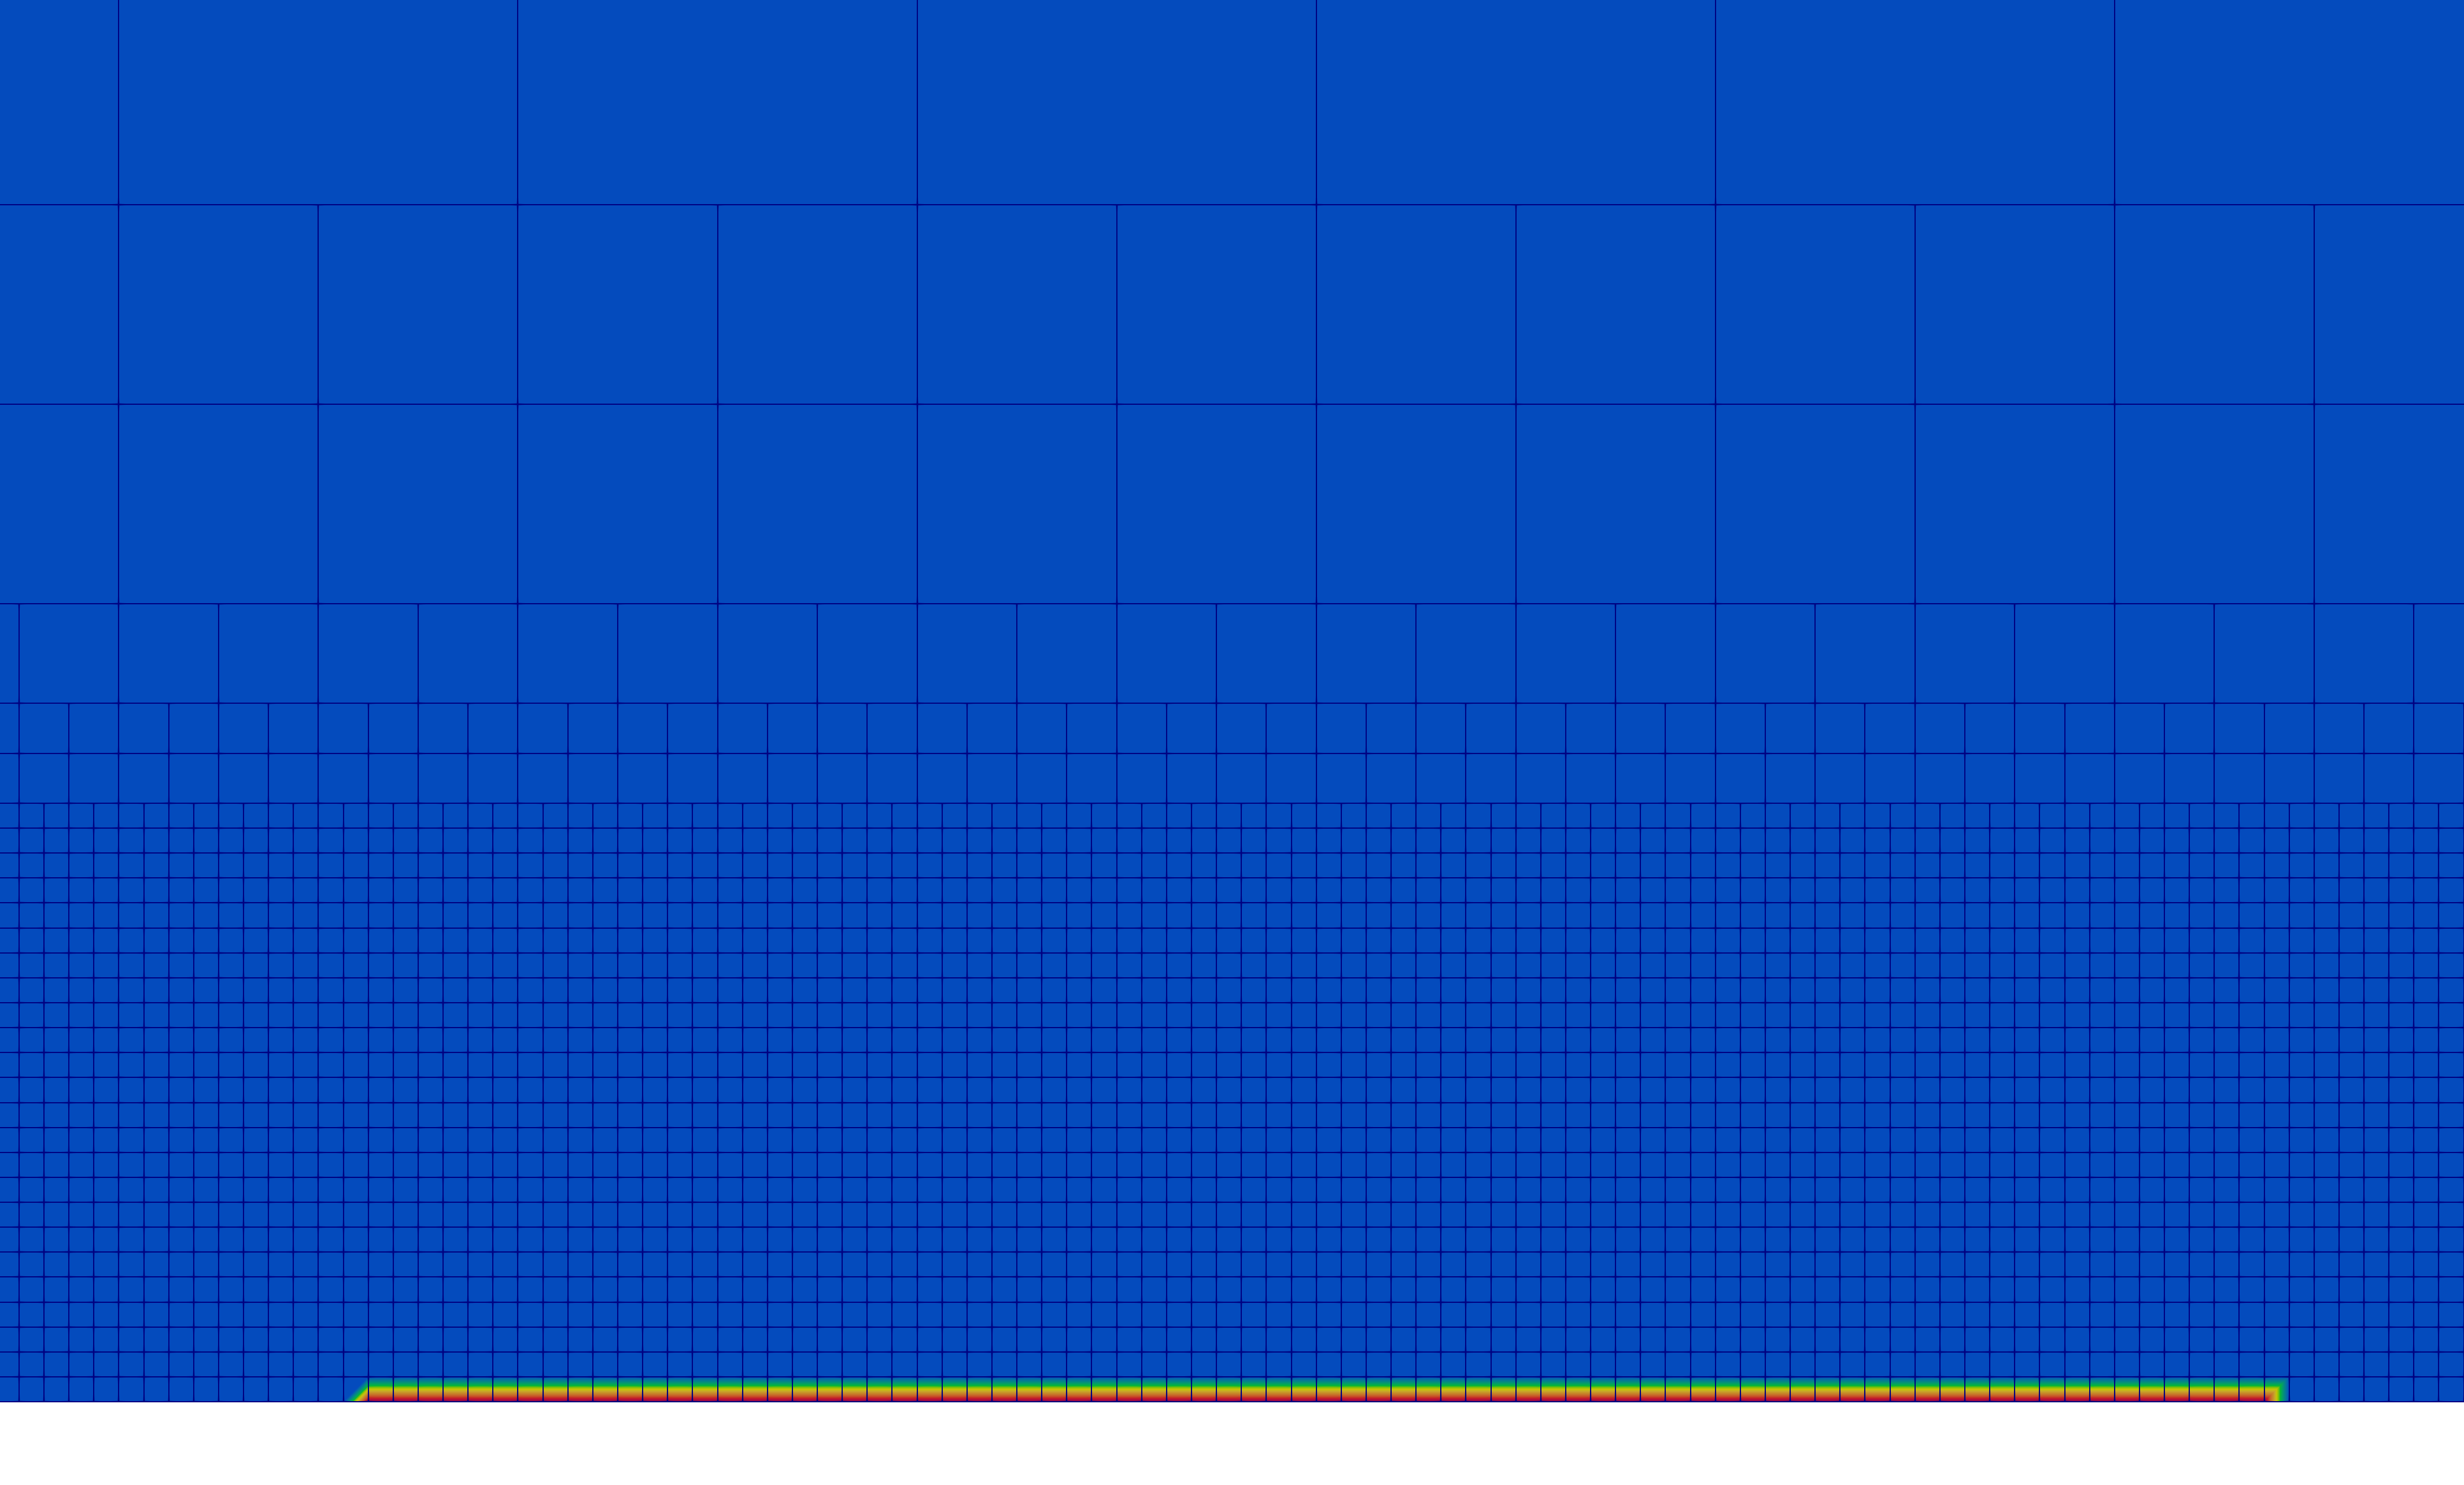
\includegraphics[width=\linewidth]{Chapter3/figures/sneddon_c0}
    \caption{}
    \label{fig:sneddon_c0}
  \end{subfigure}
  \begin{subfigure}[t]{0.46\linewidth}
    \centering
    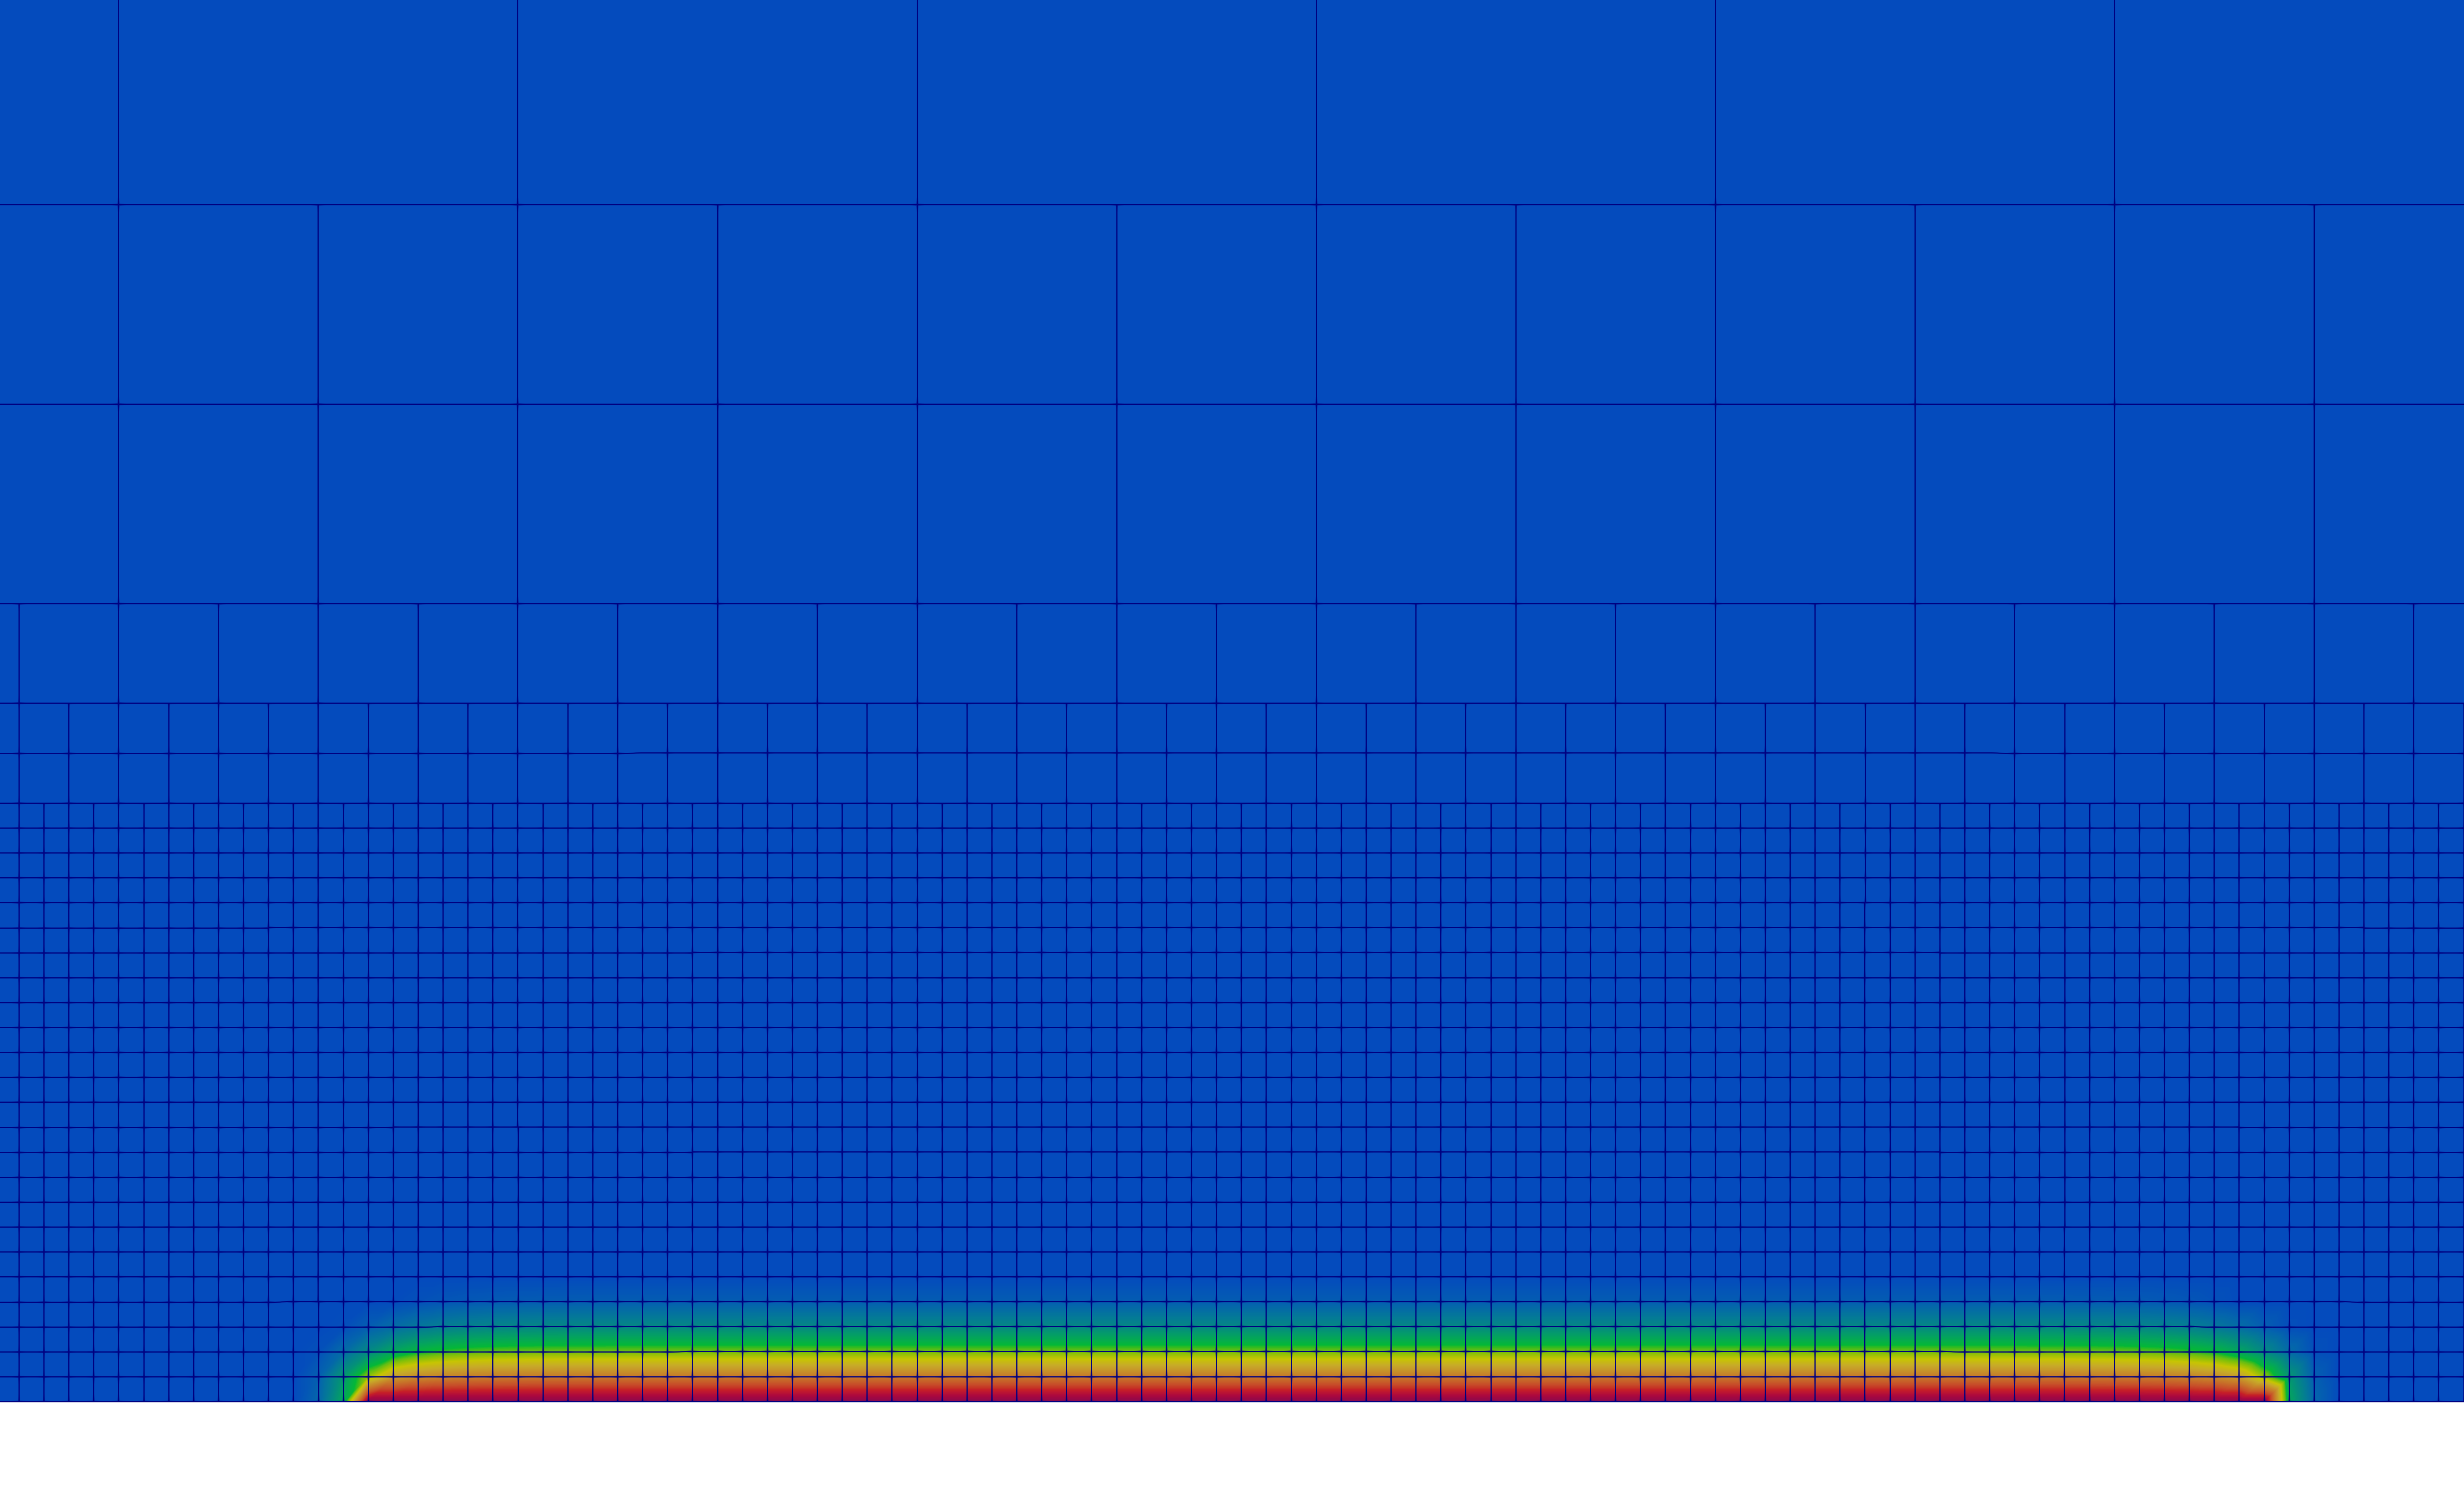
\includegraphics[width=\linewidth]{Chapter3/figures/sneddon_c1}
    \caption{}
    \label{fig:sneddon_c1}
  \end{subfigure}
  \begin{subfigure}[t]{0.475\linewidth}
    \centering
    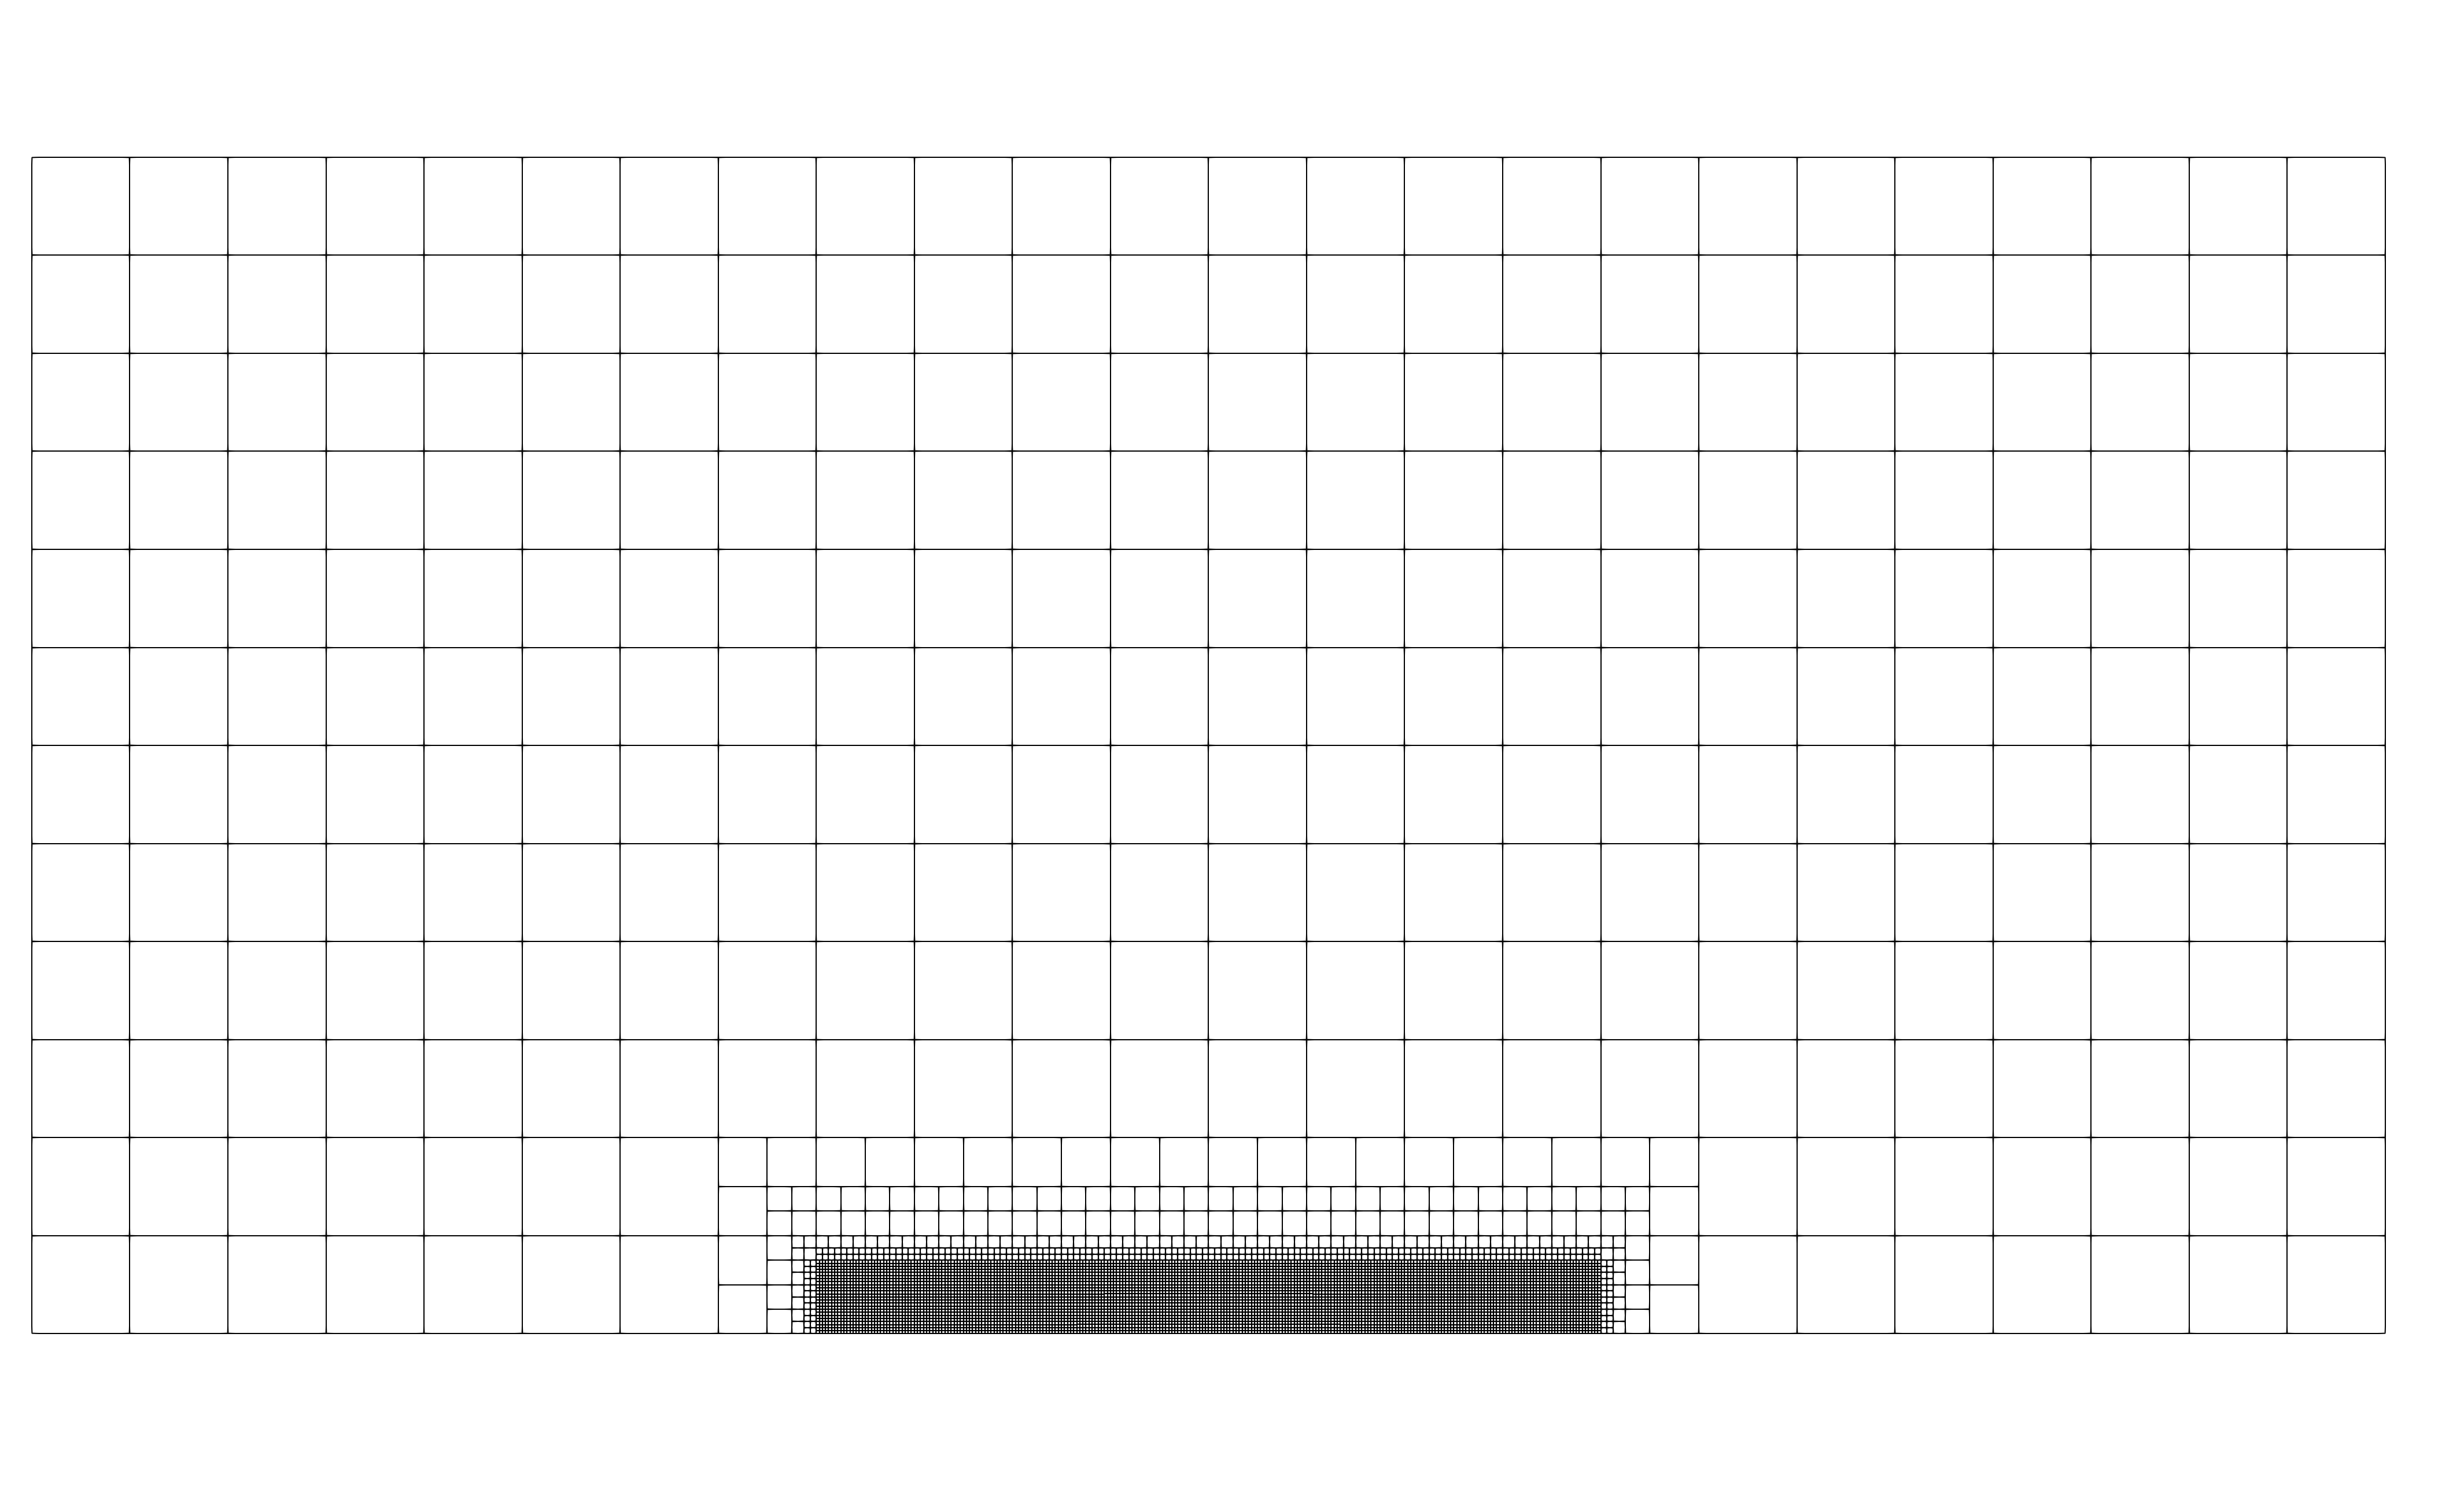
\includegraphics[width=\linewidth]{Chapter3/figures/sneddon_mesh}
    \caption{}
    \label{fig:sneddon_mesh}
  \end{subfigure}
  \begin{subfigure}[t]{0.475\linewidth}\centering
    
\includegraphics[width=\linewidth]{Chapter3/figures/sneddon_c}
    \caption{}
    \label{fig:sneddon_c}
  \end{subfigure}
  \caption[Sneddon benchmark problem.]{\label{fig:sneddon}Pressurized crack propagation problem: (a) Initial values are imposed on crack surface nodes (zoomed view). (b) Regularized phase-field variable after one time step (zoomed view). (c) Mesh with five levels of local refinement. (d) Pre-existing crack. The red and blue color correspond to value of 1 and 0, respectively.}
\end{figure}

\begin{figure}[!ht]
  \centering
  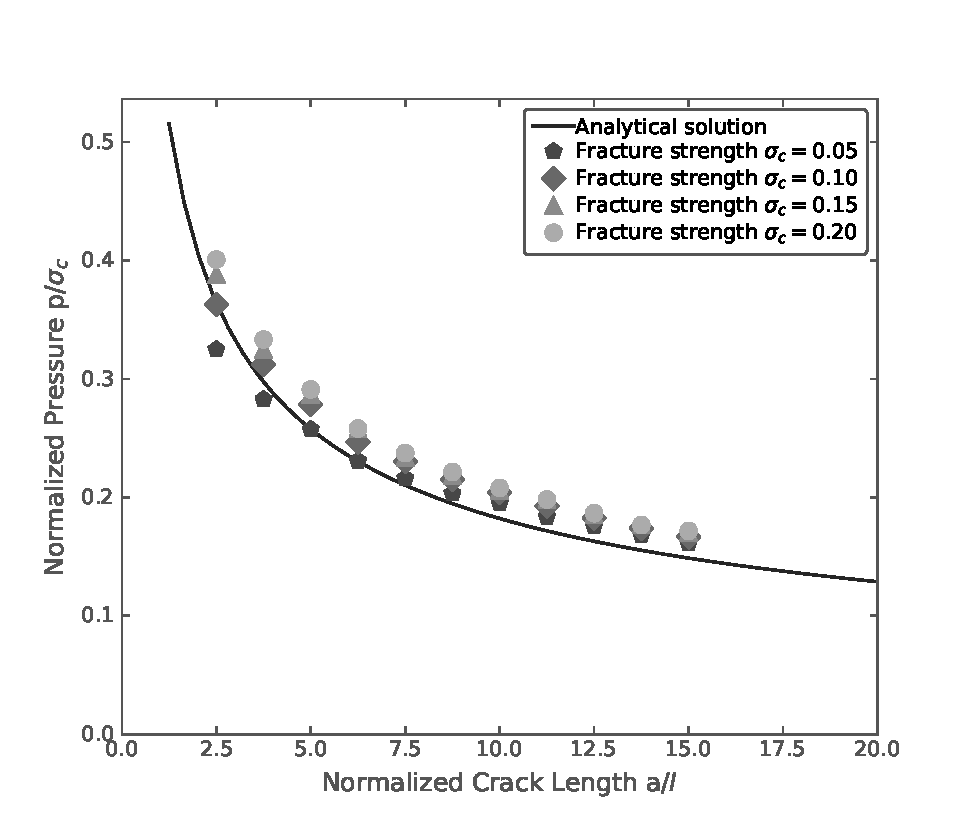
\includegraphics[width=0.6\textwidth]{Chapter3/figures/critical_pressure}
  \caption{Comparison between the numerical results and the LEFM solution for the critical pressure values.}
  \label{fig:critical_presssure}
\end{figure}
